%%%%%%%%%%%%%%%%%%%%%%%%%%%%%%%%%%%%%%%%%%%%%%%%%%%%%%%%%%%%%%%%%%%%%%%%%%%%%%%%
% DOCUMENT SPECIFICATION
%%%%%%%%%%%%%%%%%%%%%%%%%%%%%%%%%%%%%%%%%%%%%%%%%%%%%%%%%%%%%%%%%%%%%%%%%%%%%%%%
% \documentclass[twoside,a4paper]{scrartcl}        % Koma-script class
\documentclass[a4paper]{scrartcl}               % Koma-script class

%----------------------------------------------------------------------------------------
% PREAMBLE: PACKAGES AND CONFIGURATIONS
%----------------------------------------------------------------------------------------
% !TEX root = main.tex
%
% TODO: Have a clearer separation between ZHAW Thesis class and this preamble.

%%%%%%%%%%%%%%%%%%%%%%%%%%%%%%%%%%%%%%%%%%%%%%%%%%%%%%%%%%%%%%%%%%%%%%%%%%%%%%%%
% Fonts and characters
%%%%%%%%%%%%%%%%%%%%%%%%%%%%%%%%%%%%%%%%%%%%%%%%%%%%%%%%%%%%%%%%%%%%%%%%%%%%%%%%

% Support for special characters
\usepackage[utf8]{inputenc}    % Input encoding: Support non-ascii characters
\usepackage[T1]{fontenc}       % Font encoding: T1 is good choice for Europe

% Set main fonts
% Fonts catalogue: https://tug.org/FontCatalogue/
\usepackage{mathpazo}          % Use the Palatino font by default
\usepackage{beramono}          % Override the monospace/typewriter font

\usepackage{amssymb}           % Maths
\usepackage{amsmath}           % Maths 
\usepackage{numprint}          % For nicely printing large numbers
\usepackage{lmodern}           % Use LaTeX math fonts, requires T1


% ZHAW title font
% Try to load Helvetica Rounded Bold, and OpenType font.
% Loading OTF or system fonts is possible with XeLaTeX.
% If the document is compiled using pdfLaTeX, resort 
\usepackage{ifxetex}
\ifxetex
    \usepackage{fontspec}
    \newfontfamily\zhawtitlefont{Helvetica Rounded Bold}
\else
    \newcommand{\zhawtitlefont}{\scshape}
\fi

\newcommand{\boldit}[1]{\textit{\textbf{#1}}}

% Set Helvetica as the default font
\usepackage[scaled]{helvet}
\renewcommand{\familydefault}{\sfdefault}

%%%%%%%%%%%%%%%%%%%%%%%%%%%%%%%%%%%%%%%%%%%%%%%%%%%%%%%%%%%%%%%%%%%%%%%%%%%%%%%%
% Colors
%%%%%%%%%%%%%%%%%%%%%%%%%%%%%%%%%%%%%%%%%%%%%%%%%%%%%%%%%%%%%%%%%%%%%%%%%%%%%%%%

% Set up colors
\usepackage[dvipsnames]{xcolor} % Color management
% ZHAW Blue: Pantone 2945 U / R0 G100 B166
\definecolor{zhawblue}{rgb}{0.00, 0.39, 0.65}
\definecolor{zhawlightblue}{rgb}{0.82, 0.88, 0.93}
% Colors related to code listings
\definecolor{codegreen}{rgb}{0,0.6,0}
\definecolor{codegray}{rgb}{0.5,0.5,0.5}
\definecolor{codepurple}{rgb}{0.58,0,0.82}
\definecolor{codebackground}{rgb}{0.93,0.94,0.95}
% Colors related to tables
\definecolor{tablegray}{rgb}{0.9,0.9,0.9}
\colorlet{tableheader}{tablegray}
% Colors related to hyperref
\definecolor{linkcolor}{rgb}{0.1, 0.1, 0.1}

%%%%%%%%%%%%%%%%%%%%%%%%%%%%%%%%%%%%%%%%%%%%%%%%%%%%%%%%%%%%%%%%%%%%%%%%%%%%%%%%
% Environments
%%%%%%%%%%%%%%%%%%%%%%%%%%%%%%%%%%%%%%%%%%%%%%%%%%%%%%%%%%%%%%%%%%%%%%%%%%%%%%%%

\usepackage[ngerman]{babel}    % Language support

\usepackage[                    % Create hypertext links
    colorlinks=true, 
    allbordercolors={white}, 
    linkcolor=linkcolor, 
    citecolor=linkcolor, 
    filecolor=linkcolor, 
    urlcolor=linkcolor]{hyperref}

\usepackage{graphicx}          % Include graphics
\usepackage{tabularx}          % Create nicer tables
\usepackage{booktabs}          % To further beautify tables

\usepackage{caption}           % Customized caption
\usepackage{subcaption}        % Subfigure captions
\usepackage{makecell}          % Per-cell formatting in tables (\makecell)
\usepackage{pdfpages}          % Required to include PDF files/graphics (\includepdf)
\usepackage{colortbl}          % Tables with colors

\usepackage{todonotes}         % Introduces the command \todo
\setlength{\marginparwidth}{2.5cm} % Adjust this if the todo notes are out of margins
\usepackage{array,ragged2e}    % For ragged alignment of multi-line table cells

% Adjust tables
\colorlet{tableheadcolor}{gray!25}                % Table header colour
\newcommand{\headcol}{\rowcolor{tableheadcolor}}% % The color of the head
\newcommand{\topline}{\arrayrulecolor{black}      %
                      \specialrule{0.1em}{\abovetopsep}{0.5pt}%
                      \arrayrulecolor{tableheadcolor}%
                      \specialrule{\belowrulesep}{0pt}{-3pt}%
            \arrayrulecolor{black}
            }
\newcommand{\midline}{\arrayrulecolor{tableheadcolor}
            \specialrule{\aboverulesep}{-1pt}{0pt}%
            \arrayrulecolor{black}\specialrule{\lightrulewidth}{0pt}{0pt}%
            \arrayrulecolor{white}\specialrule{\belowrulesep}{0pt}{-3pt}%
            \arrayrulecolor{black}
            }
\newcommand{\bottomline}{\arrayrulecolor{white}\specialrule{\aboverulesep}{0pt}{-2pt}%
            \arrayrulecolor{black}\specialrule{\heavyrulewidth}{0pt}{\belowbottomsep}}%

% Create boxes as follows:
% \begin{colorbox}{red}{2}
\usepackage{tcolorbox}
\newtcolorbox{textbox}[2]{
    arc=3pt,
    boxrule=#2pt,
    colback=#1!25!white,
    width=\textwidth,
    halign=left,
    valign=center,
    colframe=#1!75!black
}

%%%%%%%%%%%%%%%%%%%%%%%%%%%%%%%%%%%%%%%%%%%%%%%%%%%%%%%%%%%%%%%%%%%%%%%%%%%%%%%%
% Code listings
%%%%%%%%%%%%%%%%%%%%%%%%%%%%%%%%%%%%%%%%%%%%%%%%%%%%%%%%%%%%%%%%%%%%%%%%%%%%%%%%
\captionsetup{format=plain,             % plain or hang
              justification=justified,  % justified, centering, raggedright, ...
              labelfont=bf,
              font=small,
              margin=20pt}
              

%%%%%%%%%%%%%%%%%%%%%%%%%%%%%%%%%%%%%%%%%%%%%%%%%%%%%%%%%%%%%%%%%%%%%%%%%%%%%%%%
% Code listings
%%%%%%%%%%%%%%%%%%%%%%%%%%%%%%%%%%%%%%%%%%%%%%%%%%%%%%%%%%%%%%%%%%%%%%%%%%%%%%%%

\newcommand{\code}[1]{\texttt{#1}}

% Setup code listings
\usepackage{listings}
\lstdefinestyle{mystyle}{
    backgroundcolor=\color{codebackground},   
    commentstyle=\color{codegreen},
    keywordstyle=\color{magenta},
    numberstyle=\tiny\color{codegray},
    stringstyle=\color{codepurple},
    basicstyle=\ttfamily\scriptsize,
    breakatwhitespace=false,
    breaklines=true,
%    captionpos=b,
    keepspaces=true,
    numbers=left,
    numbersep=5pt,
    showspaces=false,
    showstringspaces=false,
    showtabs=false,
    tabsize=4
}
\lstset{style=mystyle}

% minted is an alternative code listing package. (See appendix A)
% For it to run successfully, ensure the following:
% - the Python package Pygments. Install with the following command:
%       python -m pip install Pygments
% - pdflatex (or xelatex) is executed with the flag --shell-escape
%   If you are using a TEX editor, you can modify the typesetting 
%   command somewhere in the settings.
%\usepackage[outputdir=build]{minted}
%\usemintedstyle{xcode}
% For fancier coloring schemes, see here:
% https://tex.stackexchange.com/questions/585582
% One could also create an own style in Pygments
% https://pygments.org/docs/styles/#creating-own-styles


%%%%%%%%%%%%%%%%%%%%%%%%%%%%%%%%%%%%%%%%%%%%%%%%%%%%%%%%%%%%%%%%%%%%%%%%%%%%%%%%
% References
%%%%%%%%%%%%%%%%%%%%%%%%%%%%%%%%%%%%%%%%%%%%%%%%%%%%%%%%%%%%%%%%%%%%%%%%%%%%%%%%

% Set up references
\usepackage[
    backend=biber,             % Use biber backend (an external tool)
    sorting=none,              % Enumerates the reference in order of their appearance
    style=authoryear           % Choose here your preferred citation style
]{biblatex}
\addbibresource{SA1.bib} % The filename of the bibliography
\usepackage[autostyle=true]{csquotes} 
                               % Required to generate language-dependent quotes 
                               % in the bibliography


%%%%%%%%%%%%%%%%%%%%%%%%%%%%%%%%%%%%%%%%%%%%%%%%%%%%%%%%%%%%%%%%%%%%%%%%%%%%%%%%
% MARGIN SETTINGS
%%%%%%%%%%%%%%%%%%%%%%%%%%%%%%%%%%%%%%%%%%%%%%%%%%%%%%%%%%%%%%%%%%%%%%%%%%%%%%%%
\usepackage{geometry}
\geometry{
    paper=a4paper,       % Change to letterpaper for US letter
    %inner=2.5cm,        % Inner margin
    %outer=3.8cm,        % Outer margin
    %top=1.5cm,          % Top margin
    bottom=4.cm,         % Bottom margin
    bindingoffset=.5cm,  % Binding offset
    %showframe,          % Show the type block of the page
}

% Other layout settings
\setlength\parindent{0em} % No indent
\setlength{\parskip}{1em}
%\usepackage{parskip}


\setlength{\intextsep}{30pt}   % Distance between image and text 
\usepackage{enumitem}          % Layout control for list environments (e.g, itemize)
\setlist{noitemsep}            % Suppress extra spaces between items
%\setlist{nosep}               % Suppress spaces before/after list environments


%----------------------------------------------------------------------------------------
%   PENALTIES
%----------------------------------------------------------------------------------------

\doublehyphendemerits=10000 % No consecutive line hyphens
\brokenpenalty=10000 % No broken words across columns/pages
\widowpenalty=9999 % Almost no widows at bottom of page
\clubpenalty=9999 % Almost no orphans at top of page
\interfootnotelinepenalty=9999 % Almost never break footnotes


%%%%%%%%%%%%%%%%%%%%%%%%%%%%%%%%%%%%%%%%%%%%%%%%%%%%%%%%%%%%%%%%%%%%%%%%%%%%%%%%
% MANAGE AUTHOR LISTS
%%%%%%%%%%%%%%%%%%%%%%%%%%%%%%%%%%%%%%%%%%%%%%%%%%%%%%%%%%%%%%%%%%%%%%%%%%%%%%%%

\usepackage[affilmode=count]{authors}


% Trick: Convert the setter into a getter.
\NewDocumentCommand{\projecttitle}{m}{\renewcommand{\projecttitle}{#1}}
\NewDocumentCommand{\projecttype}{m}{\renewcommand{\projecttype}{#1}}
\NewDocumentCommand{\projectcode}{m}{\renewcommand{\projectcode}{#1}}
\NewDocumentCommand{\projectdate}{m}{\renewcommand{\projectdate}{#1}}
\NewDocumentCommand{\keywords}{m}{\renewcommand{\keywords}{#1}}

\NewDocumentCommand{\university}{m}{\renewcommand{\university}{#1}}
\NewDocumentCommand{\department}{m}{\renewcommand{\department}{#1}}
\NewDocumentCommand{\institute}{m}{\renewcommand{\institute}{#1}}
\NewDocumentCommand{\group}{m}{\renewcommand{\group}{#1}}


%----------------------------------------------------------------------------------------
%   HEADERS AND FOOTERS
%----------------------------------------------------------------------------------------

% Notes:
% - In twoside mode, left and right side pages may differ
% - Pages: left = even, right = odd
%   Chapters usually are forced to start at odd pages.
% - \markboth{left}{right} how left and right pages are marked
% - \automark is a convenience command from the scrlayer-scrpage package. It issues 
%   that \markboth is called for every \chapter and \section command.
% - Historical note: scrlayer-scrpage is the successor of scrpage2
% - Refs:
%    \markboth:  https://tex.stackexchange.com/questions/198676
%    \automark:  https://tex.stackexchange.com/questions/34269/
%    \automark*: https://tex.stackexchange.com/questions/348550/
%
\usepackage[markcase=used]{scrlayer-scrpage}
\ifoot{}% Empty inner footer by default
\ofoot{}% Empty outer footer by default
\providepairofpagestyles{basicStyle}{
    % Header specs for style basicStyle
    \clearpairofpagestyles%
    % \automark[section]{section}
    % \ihead{\headmark}% Inner header
    % \ohead[\pagemark]{\pagemark}% Outer header
    \cfoot[\pagemark]{\pagemark}% Footer with pagemark in the middle
}
\pagestyle{basicStyle}

\providepairofpagestyles[basicStyle]{reportStyle}{%
    \automark*[subsection]{}% Override right marks with section title once one is set
                         % Otherwise, use the chapter title -> basicStyle
}
% \pagestyle{reportStyle}

\KOMAoption{headsepline}{false} % set true to get a line below the header








% Includes for blind texts...
\usepackage{blindtext}
\usepackage{kantlipsum}

%----------------------------------------------------------------------------------------
% PROJECT INFORMATION: MODIFY THIS SECTION!
%----------------------------------------------------------------------------------------
\projecttitle{Accessibility of Ecoacoustics: A Deep Learning Approach to Insect Sound Classification}
\projecttype{Term Paper 1}
\projectcode{}
\projectdate{\today}
\keywords{ecoacoustics, bioacoustics, classification, deeplearning, machinelearning, signalprocessing, audioanalysis}

%----------------------------------------------------------------------------------------
% AUTHORS AND AFFILIATIONS
%----------------------------------------------------------------------------------------
\addauthor{A}{Julian}{Kraft}{kraftjul@students.zhaw.ch}{1}

\addcollaborator{A}{Dr. Matthias}{Nyfeler}{nife@zhaw.ch}{2}

\addaffiliation{1}
{Institute of Natural Resource Sciences}
{https://www.zhaw.ch/en/lsfm/institutes-centres/iunr/}
{3180 18th Street, San Francisco, California, USA}

\addaffiliation{2}
{Institute of Computational Life Sciences}
{https://www.zhaw.ch/en/lsfm/institutes-centres/icls/}
{Schloss 1, Wädenswil, Switzerland}

\university{Zurich University of Applied Sciences}
\department{Life Sciences and Facility Management}
\institute{Institute of Natural Resource Sciences} 
\group{} 

\AtBeginDocument{
\hypersetup{pdftitle=\projecttitle} % Set the PDF's title to your title
\hypersetup{pdfauthor=\printauthors} % Set the PDF's author to your name
\hypersetup{pdfkeywords=\keywords} % Set the PDF's keywords to your keywords
}

\begin{document}
\hypersetup{linkcolor=black, urlcolor=black} % Make links black for first part
%----------------------------------------------------------------------------------------
% TITLE PAGE AND IMPRINT
%----------------------------------------------------------------------------------------
% !TEX root = ../main.tex

%%%%%%%%%%%%%%%%%%%%%%%%%%%%%%%%%%%%%%%%%%%%%%%%%%%%%%%%%%%%%%%%%%%%%%%%%%%%%%%%
% TITLE PAGE
%%%%%%%%%%%%%%%%%%%%%%%%%%%%%%%%%%%%%%%%%%%%%%%%%%%%%%%%%%%%%%%%%%%%%%%%%%%%%%%%

% New command to make the lines in the title page
\newcommand{\HRule}{\rule{.9\linewidth}{.6pt}} 

\newgeometry{margin=1in}
\begin{titlepage}

% Make the title page mostly inert to the parskip-setting.
\setlength{\parskip}{0pt}

\begin{center}

\includegraphics[width=0.15\textwidth]{Figures/zhaw_rgb}

\ifxetex
    \vspace{0.6cm}
    {\zhawtitlefont\color{zhawblue}\LARGE\university\par}   % University
    \vspace{0.2cm}
\else
    \vspace{0.87cm}
    {
\includegraphics[height=17.9pt]{figures/zhaw_font_eng_font}\par}
    \vspace{0.05cm}
\fi
{\Large \ifdefempty{\department}{}{Department \department\par}} % Department
\vspace{0.2cm}
{\Large \institute\par}                                     % Institute
\vspace{3.5cm}                            
\textsc{\Large \projecttype}                                % Project type
\vspace{0.2cm}
\HRule 
\vspace{0.4cm}
{\huge \bfseries \projecttitle\par}                         % Project title
\vspace{0.4cm}  
\HRule
\vspace{1.5cm}



\begin{footnotesize}
\begin{tabular}{lr}

% Authors
\begin{minipage}[t]{0.41\textwidth}
\begin{flushleft}
    \boldit{Authors:}\\
    \printauthors[\\][email3]% No whitespace!
    \vspace{1cm}
\end{flushleft}
\end{minipage}

&

% Collaborators
\begin{minipage}[t]{0.41\textwidth}
\begin{flushright}
    \boldit{Collaborators:} \\
    \printcollaborators[\\][email3]% No whitespace!
    \vspace{1cm}
\end{flushright}
\end{minipage}

\\

% Affiliations
\begin{minipage}[t]{0.41\textwidth}
\begin{flushleft}
    \boldit{Affiliations:} \\
    \printaffiliations[\\]
\end{flushleft}
\end{minipage}

&

% Industrial partners
\begin{minipage}[t]{0.41\textwidth}
\begin{flushright}
    \boldit{Industry partner:} \\
    \printcompanies[\\]
\end{flushright}
\end{minipage}

\end{tabular}
\end{footnotesize}

% \begin{footnotesize}
% \begin{minipage}[t]{0.4\textwidth}
% \begin{flushleft}
%     \emph{Authors:}\\
%     \printauthors[\\][compact]\\
%     \vspace{0.5cm}
%     \emph{Affiliations:} \\
%     \printaffiliations[\\]
% \end{flushleft}
% \end{minipage}
% \begin{minipage}[t]{0.4\textwidth}
% \begin{flushright}
%     \emph{Partners:} \\
%     \printcollaborators[\\][compact]\\
%     \vspace{0.5cm}
%     \emph{Industrial partner:} \\
%     \printcompanies[\\]
% \end{flushright}
% \end{minipage}
% \end{footnotesize}

\vspace{2cm}
 
\vfill

{\large
\projectdate\\
\vspace{1.5cm}
Project Code:\\
\projectcode
}
\vfill
\end{center}
\end{titlepage}
\restoregeometry


%\let\cleardoublepage\clearpage % not needed for single-sided printing

% !TEX root = ../main.tex

%----------------------------------------------------------------------------------------
% IMPRINT
%----------------------------------------------------------------------------------------

\thispagestyle{empty}
\vspace*{\fill}

\section*{Imprint}
%\vspace{0.75cm}

\begin{footnotesize}


\begin{flushleft} 
\begin{tabular}{ @{}lp{0.6\textwidth}@{} } 
\emph{Project type:}        & \projecttype\\
\emph{Title}:               & \projecttitle\\
\emph{Code}:                & \projectcode\\
\emph{Date}:                & \projectdate\\
\emph{Keywords}:            & \keywords\\
\emph{Copyright}:           & \university\\[0.75cm]
\emph{Authors}:             & \printauthors[\newline][email2]\\
\emph{Collaborators:}       & \printcollaborators[\newline][email2]\\
\emph{Affiliations}:        & \printaffiliations[\newline]\\
                            & \printcompanies[\newline]\\
\end{tabular}
\end{flushleft}


\end{footnotesize}


%----------------------------------------------------------------------------------------
% handeling page numbering
%----------------------------------------------------------------------------------------
\clearpage
\pagenumbering{roman}
\setcounter{page}{1}

%----------------------------------------------------------------------------------------
% ABSTRACT
%----------------------------------------------------------------------------------------
% Indicate the main file. Must go at the beginning of the file.
% !TEX root = ../main.tex

%%%%%%%%%%%%%%%%%%%%%%%%%%%%%%%%%%%%%%%%%%%%%%%%%%%%%%%%%%%%%%%%%%%%%%%%%%%%%%%%
% Abstract
%%%%%%%%%%%%%%%%%%%%%%%%%%%%%%%%%%%%%%%%%%%%%%%%%%%%%%%%%%%%%%%%%%%%%%%%%%%%%%%%

\vspace*{\fill}

\section*{Abstract}
\label{abstract}

Biodiversity is rapidly declining worldwide. The first step towards understanding the causes and taking measures to counteract this trend is the development of methods and tools to quantify and monitor it. 
The biodiversity of insects is highly relevant due to their crucial role in ecosystems.
Insects contribute to processes such as pollination, decomposition, and serving as a food source for other species.
While many methods exist to monitor insects, ecoacoustics provides a non-invasive paradigm to measure species via acoustic signals.
Recently, data-driven approaches, particularly deep learning-based methods, have proven effective in detecting insect species from acoustic in situ field measurements.
These advancements offer promising new ways to understand, monitor, and protect insect populations.
This study aims to reproduce the results of a previous research on insect sound 
classification using deep learning and to assess the accessibility of this technology. 
Using the InsectSet32 dataset, which contains 335 recordings of 32 insect species, a 
convolutional neural network (CNN) with residual blocks (ResNet) was developed. 
The model was implemented and trained using the 
PyTorch framework and optimized via hyperparameter tuning. The best-performing model 
achieved an accuracy of 0.706 on the validation set and 0.649 on the test set, 
closely aligning with the original study's findings. This work demonstrates that, 
with appropriate knowledge and relatively affordable hardware, such as a regular 
gaming computer equipped with a graphics processing unit (GPU), non-experts can effectively utilize deep 
learning models for ecoacoustic applications. The study underscores the potential 
of combining ecoacoustics with artificial intelligence to advance biodiversity monitoring, 
providing a non-invasive and efficient method for large-scale environmental assessments.

\vspace*{\fill}

%----------------------------------------------------------------------------------------
% LIST OF CONTENTS/FIGURES/TABLES PAGES
%----------------------------------------------------------------------------------------

% Comment out if any of the following is not needed:
\tableofcontents  % Add main table of contents

\hypersetup{linkcolor=linkcolor, urlcolor=urlcolor}
\textbf{Code, data, logs and LaTeX source are to be found on GitHub:}\\
\url{https://github.com/juliankraft/term_paper-ecoacoustics}
\hypersetup{linkcolor=black, urlcolor=black}

\newpage
\listoffigures    % Add list of figures
\listoftables     % Add list of tables
\hypersetup{linkcolor=linkcolor, urlcolor=urlcolor} % Reset to default after TOC


%%%%%%%%%%%%%%%%%%%%%%%%%%%%%%%%%%%%%%%%%%%%%%%%%%%%%%%%%%%%%%%%%%%%%%%%%%%%%%%%
% THESIS CONTENT - CHAPTERS
%%%%%%%%%%%%%%%%%%%%%%%%%%%%%%%%%%%%%%%%%%%%%%%%%%%%%%%%%%%%%%%%%%%%%%%%%%%%%%%%

%----------------------------------------------------------------------------------------
% handeling page numbering
%----------------------------------------------------------------------------------------
\clearpage
\pagenumbering{arabic}
\setcounter{page}{1}
%\mainmatter                     % Begin numeric (1,2,3...) page numbering
%\pagestyle{reportStyle}              % Reset the page headers
% Indicate the main file. Must go at the beginning of the file.
% !TEX root = ../main.tex

%%%%%%%%%%%%%%%%%%%%%%%%%%%%%%%%%%%%%%%%%%%%%%%%%%%%%%%%%%%%%%%%%%%%%%%%%%%%%%%%
% 01-introduction
%%%%%%%%%%%%%%%%%%%%%%%%%%%%%%%%%%%%%%%%%%%%%%%%%%%%%%%%%%%%%%%%%%%%%%%%%%%%%%%%

\section{Introduction}
\label{introduction}

The loss of biodiversity is one of the most urgent issues caused by climate and land use change \autocite{cardinaleBiodiversityLossIts2012}. 
The term biodiversity is a contraction of biological diversity, which refers to the variety and variability of life forms on Earth.
In recent years, a massive decline in biodiversity has been observed, which is mainly due to human activities. 
The loss of biodiversity is a major concern because it can have a significant impact on the ecosystem and the services it provides \autocite{brondizioGlobalAssessmentReport2019}. 
In order to quantify biodiversity and monitor its changes, it is essential to have a reliable and efficient method for quantifying it.
Many traditional methods for the quantification of biodiversity are time-consuming and expensive, and they are not suitable for large-scale monitoring.
However, there are modern approaches which have the potential to monitor biodiversity fast and efficiently.

Bioacoustics, the study of sound production, dispersion and reception in animals, is a
field of research that focusses on the side of an individual species, group or community
and their interaction with each other or their environment. 
It has provided pivotal insights into the behavior and communication of animals.
Ecoacoustics, a field of research very close to bioacoustics, has a slightly different focus.
it is the study of the soundscape of an ecosystem -- the sounds produced by all living organisms in an ecosystem.
Ecoacoustics has a broad focus and is concerned with the composition of the soundscape, the temporal and spatial patterns of sound production, 
and the relationship between the soundscape and the environment. The study of biodiversity using bioacoustics
is one of its promising applications, yet there are still major challenges ahead \autocite{scarpelliMultiIndexEcoacousticsAnalysis2021}.
Among different approaches, the passive acoustic monitoring (PAM) is a promising and non-invasive approach to monitor biodiversity via sound recordings.
The PAM paradigm is currently intensely studied and advanced, and recently also paired with modern artificial intelligence (AI) methods \autocite{dengHarnessingPowerSound2023}.
Before there can be a holistic approach to the monitoring of biodiversity using ecoacoustics, some smaller steps have to be taken.

One of these steps towards the large-scale monitoting of biodiversity via PAM is the classification of the sounds of individual species or taxonomic groups.
So far, the taxonomic coverage includes birds, cetaceans and other marine mammals, bats, terrestrial mammals,
anurans, insects and fish \autocite[4]{stowellComputationalBioacousticsDeep2022}.
Birds are the most studied group of animals in the field of bioacoustics, with a
commonly known and distributed application called the "BirdNET" \autocite{kahlBirdNETDeepLearning2021}.

Recently, the applicability of a deep learning approach to classify insects was demonstrated based on an open-access dataset of a subset of insect voices \autocite{faissInsectSet32DatasetAutomatic2022}.
The subset contains members of the two groups of insects: \textit{Orthoptera} and \textit{Cicadidae}.
\textit{Orthoptera} is an order of insects that includes grasshoppers, crickets, and katydids. \autocite{capineraOrthoptera2008}
\textit{Cicadidae}, a members of the superfamily Cicadoidea Westwood are four-winged insects with sucking 
mouthparts that possess three ocelli and a rostrum that arises from the base of the head \autocite{sanbornCicadasHemipteraCicadoidea2008}.

The focus of this study is to reproduce the results of this paper and, akin to their approach, to create a model 
that can classify a subset of insects using their voices.
More specifically, the goal is to demonstrate that this technology is accessible for everyone with the basic methodological knowledge and a 
regular gaming computer with a graphic processing unit (GPU). For this purpose, a model was
constructed and trained using the same dataset as the original paper. A hyperparameter tuning was performed to find the best
configuration for the model. The results of the hyperparameter tuning were evaluated and discussed.
The best performing model was tested and evaluated for its performance and accuracy. The results were
discussed and compared to the results of the original paper.

% Indicate the main file. Must go at the beginning of the file.
% !TEX root = ../main.tex

%%%%%%%%%%%%%%%%%%%%%%%%%%%%%%%%%%%%%%%%%%%%%%%%%%%%%%%%%%%%%%%%%%%%%%%%%%%%%%%%
% 02_methods
%%%%%%%%%%%%%%%%%%%%%%%%%%%%%%%%%%%%%%%%%%%%%%%%%%%%%%%%%%%%%%%%%%%%%%%%%%%%%%%%

\section{Methods}
\label{methods}

\subsection{Dataset}%%%%%%%%%%%%%%%%%%%%%%%%%%%%%%%%%%%%%%%%%%%%%%%%%%%%%%%%%%%%

In this study, a preexisting dataset is used -- the InsectSet32 dataset \autocite{faissInsectSet32DatasetAutomatic2022}. 
The dataset includes 335 recordings of 32 insect species, totaling 57 minutes.
About half of the recordings (147) feature nine \textit{Orthoptera} species from a dataset originally compiled by Baudewijn Odé (unpublished). 
The remaining 188 recordings, from 23 \textit{Cicadidae} species, were selected from the Global Cicada Sound 
Collection on Bioacoustica \autocite{bakerBioAcousticaFreeOpen2015}, including recordings 
published in \autocites{bakerGlobalCicadaSound2015}{poppleRevisionMyopsaltaCrucifera2017}. 
Speech annotations at the beginning of many recordings led to using the last ten seconds of audio. 
Files with strong noise or multiple species were removed. The number of files per species ranges from 4 to 22, 
with durations from 40 seconds to almost 9 minutes. All files, originally with a sampling rate of at least 44.1 kHz, 
were resampled to 44.1 kHz mono WAV for consistency.
The dataset was already split into training, validation and test sets. There are two .csv files containing
the labels and the filenames of the recordings.

\subsection{Programming Language and Frameworks}%%%%%%%%%%%%%%%%%%%%%%%%%%%%%%%%%
To build and train the deep learning model, the programming language Python was used.
The Frameworks PyTorch and Lightning are widely used and powerful tools for building deep learning models.

\subsection{Deep Learning Model}%%%%%%%%%%%%%%%%%%%%%%%%%%%%%%%%%%%%%%%%%%%%%%%%%

The deep learning model used in this study is a convolutional neural network (CNN) with residual blocks \autocite[ResNet; ][]{heDeepResidualLearning2016}
illustrated in \autoref{fig:model_flow_chart}. It consists of three main parts: An input layer,
a number of stacked residual blocks and an fully connected output layer. The input layer is a convolutional layer with a kernel
size of 1 and and output channels set to the base channels (bc) -- for this experiment it was set to 8.
Note that a convolution with a kernel size of 1 is equivalent to using a fully-connected feed-forward layer.
After the convolutional layer, the input is normed with a batch normalization layer and then passed through
a ReLU activation function. Batch normalization can make the training of neural networks more robust and faster, 
and the ReLU activation introduces non-linearity \autocite{Goodfellow-et-al-201}.
The output is than passed trough a number of residual blocks, where
Residual connections facilitate the training of deep neural networks by enabling smoother flow of gradients 
during backpropagation, i.e., the backward pass performed to compute the model gradients \autocite{Goodfellow-et-al-201}. 
The model is implemented dynamically, so the number of residual blocks can be set as a hyperparameter. Each residual block
consists of two convolutional layers, each followed by a batch normalization layer and a ReLU activation function.
The output channels are doubled with every residual block.
The residual connection is implemented by passing the input trough a separated convolutional layer with a kernel size of 1
and the same number of output channels as the output of the convolutional layers in the residual block to
match dimensions. This output is than added to the output of the transformation in the residual block.
At the end of the residual block, the output is passed trough a max pooling layer to reduce the dimensions.
The max pooling layer is implemented to alter the kernel size with every residual block. For every odd residual block
the kernel size is set to n\_max\_pool -- in this experiment it was set to 3 -- reducing the dimensions by a factor of 3.
For every even residual block the kernel size is set to 1, so the dimensions stay the same. The output of the residual blocks
is passed through a dynamic global average pooling layer, and then passed through a fully-connected feed-forward layer. An additional
convolutional layer with kernel size 1 to match the number of classes. The output was flattened and passed through a 
softmax activation function to get the probabilities for each class as a vector of length 
n\_classes -- in this experiment 32 -- elements between 0 and 1 that sum up to 1.

\subsection{Data Processing}%%%%%%%%%%%%%%%%%%%%%%%%%%%%%%%%%%%%%%%%%%%%%%%%%%%%
A custom Dataloader was implemented, to handle the data processing on the fly
and provide the trainer with then data samples matching the chosen indices.
To implement the dataloader, the PyTorch Dataset and DataLoader classes where used.
For the data processing, the torchaudio and numpy libraries where used.
There is two steps to the data processing: Sampling and Transformation.

\subsubsection{Sampling}%%%%%%%%%%%%%%%%%%%%%%%%%%%%%%%%%%%%%%%%%%%%%%%%%%%%%%%
The audio files are of different lengths and the model was fed with consistent, potentially zero-padded samples for consistency.
Since the smallest files are of a length of around 1 second and the longest file is around
160 seconds, a compromise had to be made. On the one hand, trimming the files to a length of 1 second
would mean very little information being available for the model to learn from. On the other
hand, if the files are sampled for a length of more than a second, the short files would need
to be padded with zeros meaning the file starts with an empty part. This could lead
to the model learning from the length of the empty part and not the actual audio signal, i.e., it would be prone to overfitting.
To avoid this, the audio files where sampled to a random length between 1 and 10 seconds and
then padded with zeros to the fixed length of 10 seconds. To implement this, a custom method
was implemented as shown in \autoref{lst:sampling}.

%==== listing: sampling ====%
\begin{lstlisting}[
    language=Python, 
    caption={Python code for the sampling of the filies}, 
    label={lst:sampling}]
import numpy as np
import torch

def get_random_part_padded(self, waveform: Tensor, samplerate: int) -> Tensor:

    min_len_in_samples = int(self.min_len_in_seconds * samplerate)
    max_len_in_samples = int(self.max_len_in_seconds * samplerate)

    if self.min_len_in_seconds == -1:
        sample_start_index = -max_len_in_samples
        sample_end_index = None

    else:
        part_length = np.random.randint(min_len_in_samples, max_len_in_samples + 1)
        sample_length = waveform.shape[1]
        part_length = min(part_length, sample_length)
        sample_start_index = np.random.randint(0, sample_length - part_length + 1)
        sample_end_index = sample_start_index + part_length

    waveform_part = waveform[:, sample_start_index:sample_end_index]
    actual_part_length = waveform_part.shape[1]
    pad_length = max_len_in_samples - actual_part_length
    waveform_pad = torch.nn.functional.pad(waveform_part, pad=(pad_length, 0, 0, 0))

    return waveform_pad
\end{lstlisting}
%===========================%

\subsubsection{Transformation}%%%%%%%%%%%%%%%%%%%%%%%%%%%%%%%%%%%%%%%%%%%%%%%%%%
Audio signals are rich in information, but also contain spurious information.
One way to condense the the information content of audio data is the transformation via spectrograms.
A spectrogram is constructed using short time Fourier transformation (STFT).
The STFT applies a mathematical transformation to short windows in the time domain, and transfers them from the time into the frequency domain.
The transformed snippets are aligned along the time dimension, and thereby, we obtain a two-dimensional, compressed version of the original audio signal.
As an extension of the plain spectrogram, the Mel spectrogram enhances certain frequencies, 
such that it reflects the frequencies which are perceived stronger by the the human ear, which is more sensitive to low frequencies.
This transformation is commonly used in the field of ecoacoustics \autocite[7]{stowellComputationalBioacousticsDeep2022}.
A visualization of the two transformation -- the plain spectrogram, and the Mel spectrogram---is provided in \autoref{fig:compare_spectrogram}
for a random sample with no padding. Both versions of the transformation where transformed into decibels and normalized before 
being passed into the model.
To implement the two varieties of the transformation, the library torch and torchaudio where used.
A custom transformation method was implemented, that can be used as a layer in the model as shown in 
\autoref{lst:transformation}. Some of the parameters of the transformation where made configurable
and others dependant on them where calculated. In the hyperparameter tuning phase, the only parameter
that was tuned was the number of mel bins, which was set to either 64 to use the mel-spectrogram or -1
to use the standard spectrogram.

%==== listing: transformation ====%
\begin{lstlisting}[
    language=Python, 
    caption={Python code for the transformation of the audio signal}, 
    label={lst:transformation}]
import torch
import torchaudio

class NormalizeSpectrogram(torch.nn.Module):
    def forward(self, tensor):
    return (tensor - tensor.min()) / (tensor.max() - tensor.min())

normalize_transform = NormalizeSpectrogram()

if n_mels == -1:
    spectrogram = torchaudio.transforms.Spectrogram(
        n_fft=n_fft, 
        hop_length=int(n_fft/2), 
        win_length=n_fft)
else:
    spectrogram = torchaudio.transforms.MelSpectrogram(
        n_fft=n_fft,
        hop_length=int(n_fft/2),
        win_length=n_fft,
        n_mels=n_mels,
        f_max=self.sample_rate / 2)

db_transform = torchaudio.transforms.AmplitudeToDB(top_db=top_db)

self.transform = torch.nn.Sequential(
    spectrogram, 
    db_transform, 
    normalize_transform)
\end{lstlisting}
%=================================%

\subsection{Fitting the Model}%%%%%%%%%%%%%%%%%%%%%%%%%%%%%%%%%%%%%%%%%%%%%%%%%%

The training was handled by the PyTorch Lightning framework. The logging was done
with the TensorBoard logger and with an additional custom logger to get easier access to the
data afterwards. The hyperparameter grid search was implemented with a custom Python script.

\subsubsection{Training}%%%%%%%%%%%%%%%%%%%%%%%%%%%%%%%%%%%%%%%%%%%%%%%%%%%%%%%%

The training was done on a single GPU. The model was trained for a maximum of 2000 epochs
with an early stopping callback, that stopped the training if the validation loss did not improve
for a patience of 100 epochs and the best model was restored. The model was trained with a batch size of 10. The optimizer used was the AdamW
optimizer of the PyTorch library with a weight decay of 0. The loss function used was the
CrossEntropyLoss function of the PyTorch library with default parameters and class weights
inversely proportional to the available data per class, in order to give more emphasis to classes with fewer samples. 
Different learning rates where evaluated during the hyperparameter
tuning referred to in \autoref{hyperparameter_tuning}. Only the best model was saved and used for
the evaluation of the model. In order to simplify the evaluation, on completion of the training
the whole dataset was predicted and saved to a csv file in the log folder.

\subsubsection{Hyperparameter Tuning}%%%%%%%%%%%%%%%%%%%%%%%%%%%%%%%%%%%%%%%%%%%
\label{hyperparameter_tuning}

For the hyperparameter tuning, a select number of hyperparameters where chosen to be tuned.
Considerations like the experience of some early tests, the computational resources available
and the time frame of the project where taken into account. The hyperparameters that where
chosen for the grid search are shown in \autoref{tab:hyperparameters}. For the grid search,
models for all possible combinations of the hyperparameters -- in this case \( 2 \times 3 \times 2 \times 3 = 36 \) 
where trained. To implement the grid search a short Python
script was written to create the system commands to start the training with the different
hyperparameter combinations.

%==== table: hyperparameters ====%
\begin{table}[h]
    \centering
    \caption{Hyperparameters and values used for the grid search.}
    \label{tab:hyperparameters}
    \begin{tabular}{llll}
    \toprule
    \textbf{Hyperparameter} & \textbf{Description}                  & \textbf{Variations}   & \textbf{Values} \\
    \midrule
    n\_mels                 & transformation (-1 for regular STFT)  & 2                     & 64, -1 \\
    n\_res\_blocks          & number of res blocks                  & 3                     & 2, 3, 4 \\
    learning\_rate          & step size during optimization         & 2                     & 0.001, 0.0001 \\
    kernel\_size            & dimension of the filter               & 3                     & 3, 5, 7 \\
    \bottomrule
\end{tabular}

\end{table}
%================================%

\subsection{Evaluation}%%%%%%%%%%%%%%%%%%%%%%%%%%%%%%%%%%%%%%%%%%%%%%%%%%%%%%%%%

The models were evaluated based on the predictions performed at the end of the training.
The output of the model was a vector of length 32 with probabilities for each class, which where
transformed into a predicted class ID by taking the index of the highest probability
using the argmax function of the numpy library. For all the models they where stored in a csv file
in their log folder. To evaluate the hyperparameter tuning, the predictions of the validation set
where used, as they where not used during the training of the model except for the early stopping
and the selection of the best model. To evaluate the best model, only the predictions of the test set
where used.

\subsubsection{Metrics and Tests}

\textbf{Accuracy:} The accuracy is the ratio of correctly predicted observations to the total observations.
It was calculated using the mean function of the numpy library:\\ 
\lstinline{np.mean(y_true == y_pred)}
The accuracy was the metric chosen to select the best model for further evaluation.
Note that the accuracy can be misleading, as it does not take into account class imbalances, 
and it is possible to achieve a high accuracy overall while incorrectly classifying classes with fewer samples.

\textbf{F1 Score:} The F1 score is a metric that combines the precision and recall of a model. In this
case the macro average was used, which calculates the F1 score for each class and then takes the mean.
It was calculated using the f1\_score function of the sklearn library:\\ 
\lstinline{f1_score(y_true, y_pred, average='macro', sample_weight=None, zero_division='warn')}

\textbf{F1 Score per Class:} The F1 score per class was calculated
using the f1\_score function of the sklearn library with the average parameter set to None:\\
\lstinline{f1_score(y_true, y_pred, average=None, sample_weight=None, zero_division='warn')}\\
It was calculated for each class and for each model from the hyperparameter tuning. The results
where than aggregated to get the mean F1 score per class over all models.

\textbf{Confusion Matrix:} The result of the Predictions of the best model where used to create a confusion matrix.
The confusion matrix is a table that is often used to analyze the performance of a classification model.
Predictions and true labels are compared and visualized in a matrix it was calculated using the 
confusion\_matrix function of the sklearn library.

\textbf{Pearson Test:} The Pearson test was used to test the correlation between the model size and the accuracy
or F1 score of the models. The Pearson test was calculated using the pearsonr function of the scipy library:\\
\lstinline{for i, metric in enumerate(['accuracy', 'f1']):}\\
\lstinline{  pearson_corr, p_value = stats.pearsonr(ex.summary[metric], ex.summary['num_trainable_params'])}\\
And the correlation between the train data count and the F1 score per class:\\
\lstinline{pearson_corr, p_value = stats.pearsonr(data['f1'], data['count'])}\\
For both cases the null hypothesis (H0) posited that there is no correlation, with the significance level (alpha) set at 0.05.

%==== figure: compare_spectrogram ====%
\begin{figure}[h]
\centering
\captionsetup{width=0.8\linewidth}
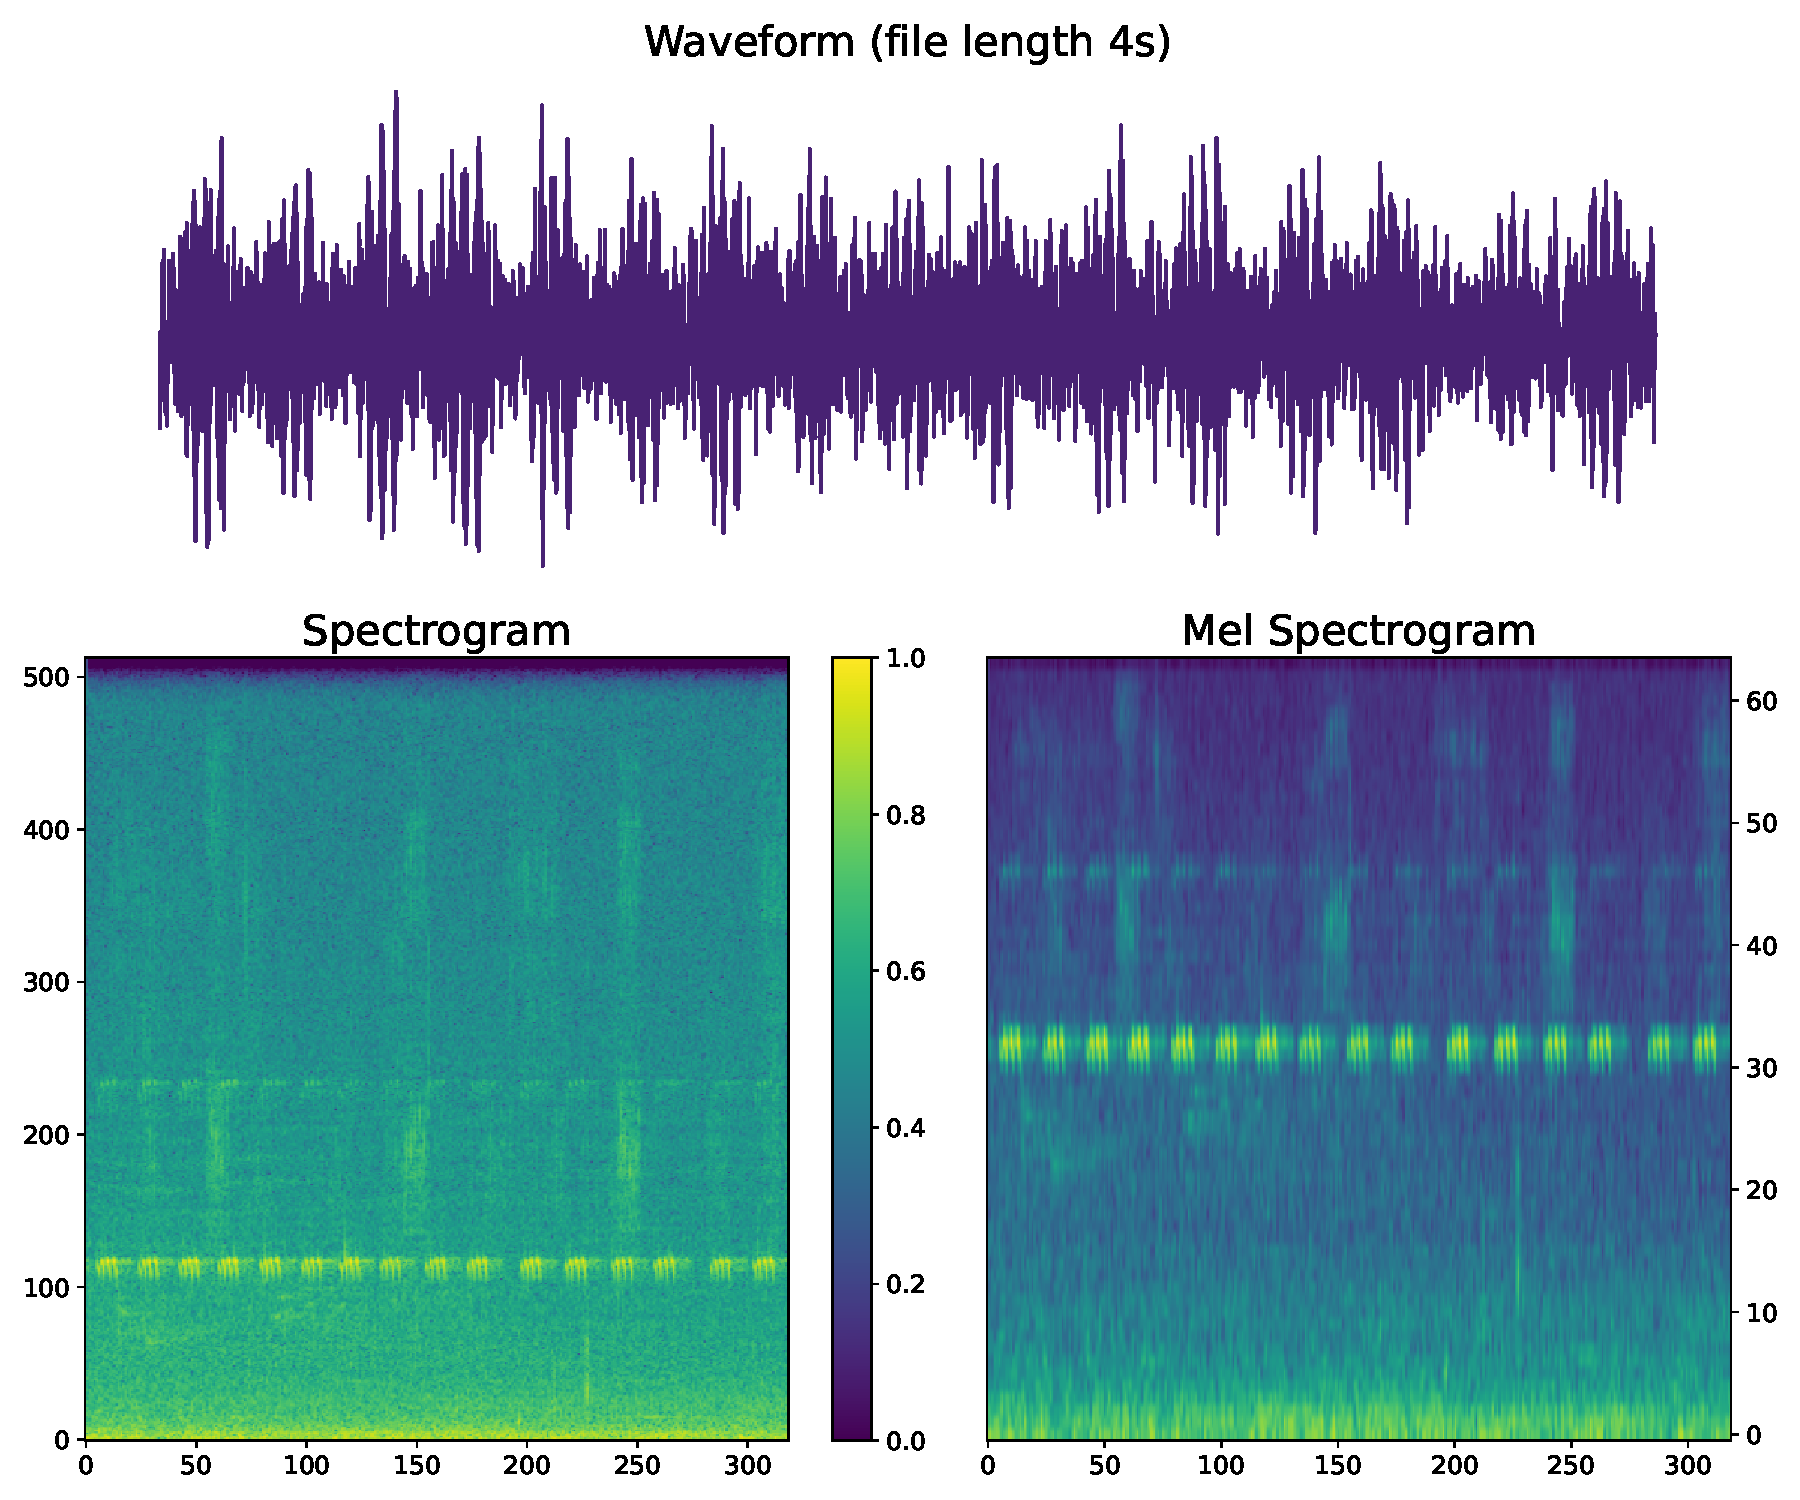
\includegraphics{figures/compare_spectrogram.pdf}
\caption{Visualization of the two transformations of the audio signal.}
\label{fig:compare_spectrogram}
\end{figure}

%=====================================%

%==== figure: model_flow_chart ====%
\begin{figure}[h]
    \centering
    \captionsetup{width=.9\linewidth}
    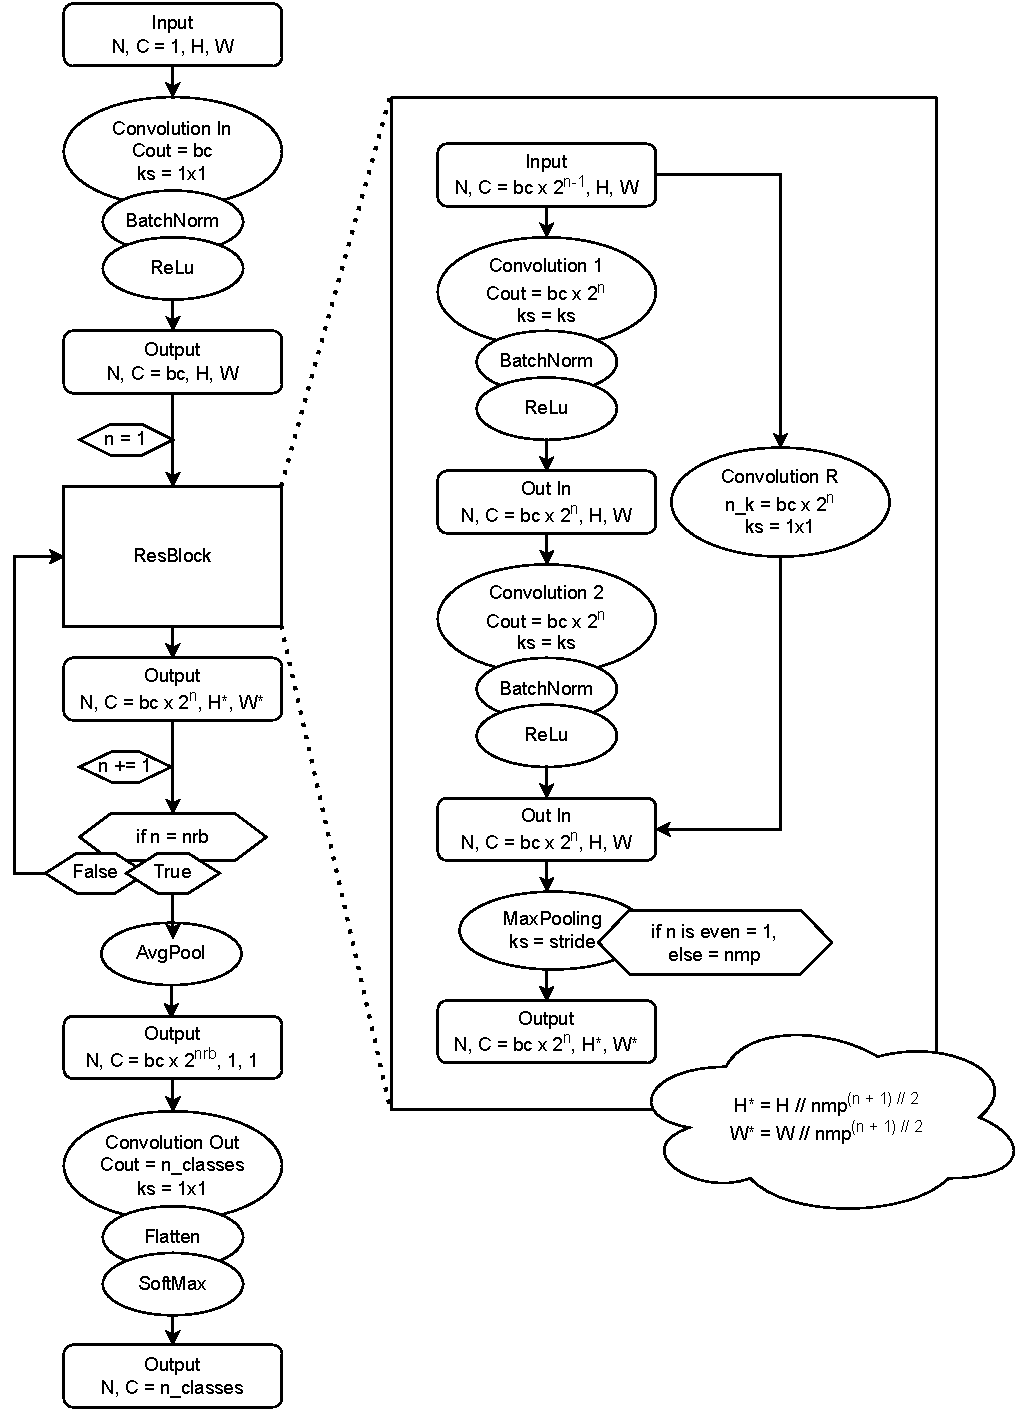
\includegraphics[width=1\textwidth]{figures/model_flow_chart.pdf}
    \caption{
        Flow chart illustrating the models architecture. N: elements in batch, C: channels, H: height, W: width,
        Cout: output channels, ks: kernel size, bc: base channels, nrb: number of residual blocks,
        n\_classes: number of classes, nmp: parameter for max pooling
        }
    \label{fig:model_flow_chart}
\end{figure}
%==================================%
% Indicate the main file. Must go at the beginning of the file.
% !TEX root = ../main.tex

%%%%%%%%%%%%%%%%%%%%%%%%%%%%%%%%%%%%%%%%%%%%%%%%%%%%%%%%%%%%%%%%%%%%%%%%%%%%%%%%
% SECTION 3
%%%%%%%%%%%%%%%%%%%%%%%%%%%%%%%%%%%%%%%%%%%%%%%%%%%%%%%%%%%%%%%%%%%%%%%%%%%%%%%%


\section{Results}
\label{section3}

% Indicate the main file. Must go at the beginning of the file.
% !TEX root = ../main.tex

%%%%%%%%%%%%%%%%%%%%%%%%%%%%%%%%%%%%%%%%%%%%%%%%%%%%%%%%%%%%%%%%%%%%%%%%%%%%%%%%
% 04_discussion
%%%%%%%%%%%%%%%%%%%%%%%%%%%%%%%%%%%%%%%%%%%%%%%%%%%%%%%%%%%%%%%%%%%%%%%%%%%%%%%%


\section{Discussion}
\label{discussion}

\subsection{Hyperparameter Tuning}%%%%%%%%%%%%%%%%%%%%%%%%%%%%%%%%%%%%%%%%%%%%%%

The detailed results of the hyperparameter tuning are shown in \autoref{tab:hyperparameters_results}.
It is quite difficult to find any obvious tendencies for the influence of the
hyperparameters on the performance of the model. There is no direct correlation
between the model size and the performance of the model. This might be explicable
by the fact that the available data is not sufficient to train larger models
This could be helped by extending the dataset with additional recordings or by
implementing some sort of data augmentation \autocite[3]{stowellComputationalBioacousticsDeep2022}. 
Some ideas being to add random levels of noise to the recordings or to randomly add slight shifts in time or frequency.
An other approach could be to mix data from different classes to create new samples.
This would have two main advantages. First, the combination possibilities are nearly endless
and therefore the dataset could be extended massively. Second, the model would be
trained to to detect multiple classes in one sample wich could be useful in a real
world scenario where multiple species are present at the same time.
The data augmentation could be implemented in the dataloader to be done on the fly.

An other aspect to look into is the selection of the hyperparameters. Due to limited
resources, the hyperparameter tuning was done with a limited number of configurations.
There is still a list of potential hyperparameters that could be tested. As an example,
the base channels after the input layer, or different parameters for the transformation
such as the hop length, window size or the number of mel bins could be further investigated. As the model is, the
kernel size stays constant for all layers -- the possibilities there are endless.
Furthermore, other deep learning architectures could be explored. 
It is possible that -- given the low amount of training samples -- a smaller 
and more efficient model architecture could perform better than the ResNet used here.

\subsection{Comparison of Results with Original Study}%%%%%%%%%%%%%%%%%%%%%%%%%%

In the original paper \autocite{faissAdaptiveRepresentationsSound2023},
different datasets and models were evaluated. The model was
run five times with different seeds and the accuracy was averaged to achieve an ensemble of predictions, 
which can be more robust. The model using a MelSpectrogram
frontend on the InsectSet32 dataset achieved an mean accuracy of 0.6 with a range of 0.57 to 0.65
on the validation set and an accuracy of 0.62 with a range of 0.57 to 0.67 on the test set.
The best performing configuration for the model in this study achieves an accuracy of 0.706 on the validation set
and an accuracy of 0.649. For the test set, this is well in the range of the original paper.
Why the model in this study performs better on the validation set compared to the difference
between the validation and test set in the original paper is not clear. The accuracy achieved
by the model with the other frontend from the original paper is unreached by the model in this study.
Consequently, there is still room for improvement especially in the data processing and, as already mentioned, data augmentation.

\subsection{Conclusion}%%%%%%%%%%%%%%%%%%%%%%%%%%%%%%%%%%%%%%%%%%%%%%%%%%%%%%%%%

Species classification with deep learning can support the non-invasive monitoring of biodiversity.
However, the advanced methodological approaches and computation demands needed for such endeavors can be an obstacle.
In this study, I reproduced a prior study on classifying insects based on an open-access dataset.
I wanted to investigate whether the results can be replicated with limited technical knowhow, 
computational resources, and under temporal constraints.
The model was trained on a regular gaming computer with a GPU by a student with none to little experience
in the field of deep learning -- notable with quite some demand for support (refer to Acknowledgments \ref{acknowledgment_declaration}).
Still, it is save to say that this technology has become broadly accessible.
The model performance was comparable to the original study in terms of accuracy.
The model was able to classify the sounds of a limited subset of insects with an accuracy of 0.649.
I identified some shortcomings of the approach:
The training dataset is rather small, and additional samples could potentially improve the results further.
Similarly, data augmentation could enhance the classification skill.
I encourage the investigation of additional deep learning model architectures and 
an an exhaustive sampling of the hyperparameter space to further improve model performance.

% Indicate the main file. Must go at the beginning of the file.
% !TEX root = ../main.tex

%%%%%%%%%%%%%%%%%%%%%%%%%%%%%%%%%%%%%%%%%%%%%%%%%%%%%%%%%%%%%%%%%%%%%%%%%%%%%%%%
% 05_acknowledgment_declaration
%%%%%%%%%%%%%%%%%%%%%%%%%%%%%%%%%%%%%%%%%%%%%%%%%%%%%%%%%%%%%%%%%%%%%%%%%%%%%%%%


\section{Acknowledgment and Declaration}
\label{acknowledgment_declaration}

\subsection{Acknowledgment}%%%%%%%%%%%%%%%%%%%%%%%%%%%%%%%%%%%%%%%%%%%%%%%%%%%%%%

I thank Dr. Matthias Nyfeler for his support and the many interesting discussions we had.
I would like to express my gratitude to my brother, Dr. Basil Kraft, for his continuous
support with his expertise in the field of machine learning. 

\subsection{Declaration of AI Usage}%%%%%%%%%%%%%%%%%%%%%%%%%%%%%%%%%%%%%%%%%%%%%%

GitHub Copilot was used to assist writing the code and text for this project.

ChatGPT was used to assist researching as well as writing the code and text for this project.

\newpage
\refstepcounter{subsection}
\addcontentsline{toc}{subsection}{\protect\numberline{\thesubsection}Statement of Authorship}


\newgeometry{left=0in, right=0in, top=0.5in, bottom=0in}
\thispagestyle{empty}
\begin{figure}[h!]
    \centering
    
\includegraphics[width=1\textwidth]{figures/denlaration_independence.pdf}
\end{figure}
\restoregeometry % Restore original margins


\printbibliography[heading=bibintoc]

\appendix
% Indicate the main file. Must go at the beginning of the file.
% !TEX root = ../main.tex

%%%%%%%%%%%%%%%%%%%%%%%%%%%%%%%%%%%%%%%%%%%%%%%%%%%%%%%%%%%%%%%%%%%%%%%%%%%%%%%%
% SECTION A (Appendix)
%%%%%%%%%%%%%%%%%%%%%%%%%%%%%%%%%%%%%%%%%%%%%%%%%%%%%%%%%%%%%%%%%%%%%%%%%%%%%%%%


\section{Appendix: Tables}
\label{apendix_tables}

\begin{table}[ht]
    \centering
    \caption{Results of the hyperparameter tuning by descending accuracy.}
    \label{tab:hyperparameters}


    \renewcommand{\arraystretch}{0.8}
    \scriptsize
    \begin{table}[H]
\centering
\captionsetup{width=0.8\linewidth}
\caption{Results of the hyperparameter tuning by descending accuracy.}
\label{tab:hyperparameters_results}
\scriptsize
\begin{tabular}{rrrrrrrr}
\toprule
\textbf{n\_mels} & \textbf{res blocks} & \textbf{learning rate} & \textbf{kernel size}& \textbf{parameters} & \textbf{epochs} & \textbf{accuracy} & \textbf{F1} \\
\midrule
64 & 4 & 0.001 & 5 & 832,912 & 1018 & 0.706 & 0.571 \\
-1 & 4 & 0.0001 & 5 & 832,912 & 672 & 0.686 & 0.557 \\
-1 & 4 & 0.0001 & 3 & 310,544 & 891 & 0.667 & 0.608 \\
-1 & 3 & 0.001 & 5 & 207,376 & 394 & 0.627 & 0.553 \\
-1 & 2 & 0.0001 & 7 & 96,528 & 1198 & 0.627 & 0.511 \\
-1 & 2 & 0.001 & 5 & 50,256 & 640 & 0.608 & 0.495 \\
-1 & 3 & 0.0001 & 7 & 401,104 & 760 & 0.608 & 0.512 \\
-1 & 3 & 0.0001 & 3 & 78,224 & 897 & 0.588 & 0.558 \\
64 & 4 & 0.0001 & 5 & 832,912 & 371 & 0.588 & 0.491 \\
64 & 3 & 0.0001 & 7 & 401,104 & 536 & 0.588 & 0.513 \\
64 & 3 & 0.001 & 7 & 401,104 & 350 & 0.588 & 0.399 \\
64 & 3 & 0.001 & 5 & 207,376 & 505 & 0.569 & 0.488 \\
-1 & 2 & 0.001 & 3 & 19,408 & 469 & 0.569 & 0.431 \\
-1 & 4 & 0.001 & 3 & 310,544 & 562 & 0.569 & 0.493 \\
64 & 3 & 0.0001 & 3 & 78,224 & 1115 & 0.529 & 0.453 \\
64 & 2 & 0.001 & 5 & 50,256 & 661 & 0.529 & 0.409 \\
64 & 2 & 0.0001 & 3 & 19,408 & 1354 & 0.529 & 0.365 \\
64 & 4 & 0.0001 & 7 & 1,616,464 & 273 & 0.510 & 0.419 \\
64 & 2 & 0.001 & 3 & 19,408 & 455 & 0.510 & 0.364 \\
-1 & 4 & 0.0001 & 7 & 1,616,464 & 296 & 0.490 & 0.394 \\
-1 & 2 & 0.0001 & 3 & 19,408 & 1138 & 0.490 & 0.350 \\
64 & 4 & 0.001 & 3 & 310,544 & 408 & 0.490 & 0.348 \\
-1 & 3 & 0.001 & 3 & 78,224 & 456 & 0.471 & 0.356 \\
-1 & 3 & 0.0001 & 5 & 207,376 & 531 & 0.451 & 0.342 \\
64 & 4 & 0.0001 & 3 & 310,544 & 330 & 0.451 & 0.308 \\
64 & 3 & 0.001 & 3 & 78,224 & 474 & 0.451 & 0.322 \\
64 & 2 & 0.0001 & 5 & 50,256 & 892 & 0.431 & 0.326 \\
64 & 3 & 0.0001 & 5 & 207,376 & 395 & 0.412 & 0.307 \\
-1 & 2 & 0.001 & 7 & 96,528 & 375 & 0.392 & 0.240 \\
64 & 4 & 0.001 & 7 & 1,616,464 & 403 & 0.353 & 0.207 \\
64 & 2 & 0.001 & 7 & 96,528 & 229 & 0.353 & 0.230 \\
64 & 2 & 0.0001 & 7 & 96,528 & 545 & 0.333 & 0.278 \\
-1 & 4 & 0.001 & 5 & 832,912 & 290 & 0.294 & 0.174 \\
-1 & 3 & 0.001 & 7 & 401,104 & 268 & 0.275 & 0.164 \\
-1 & 2 & 0.0001 & 5 & 50,256 & 432 & 0.255 & 0.109 \\
-1 & 4 & 0.001 & 7 & 1,616,464 & 145 & 0.235 & 0.151 \\
\bottomrule
\end{tabular}

\normalsize
\end{table}


    \normalsize
    \renewcommand{\arraystretch}{1.0}
    
\end{table}

\begin{table}[ht]
    \centering
    \caption{ClassID legend.}
    \label{tab:ClassID_legend}


    \renewcommand{\arraystretch}{0.8}
    \begin{table}[h]
\centering
\captionsetup{width=0.9\linewidth}
\caption{ClassID legend.}
\label{tab:ClassID_legend}
\scriptsize
\begin{tabular}{rlrl}
\toprule
ClassID & Species & ClassID & Species \\
\midrule
0 & Azanicadazuluensis & 16 & Platypleurachalybaea \\
1 & Brevisianabrevis & 17 & Platypleuradeusta \\
2 & Chorthippusbiguttulus & 18 & Platypleuradivisa \\
3 & Chorthippusbrunneus & 19 & Platypleurahaglundi \\
4 & Grylluscampestris & 20 & Platypleurahirtipennis \\
5 & Kikihiamuta & 21 & Platypleuraintercapedinis \\
6 & Myopsaltaleona & 22 & Platypleuraplumosa \\
7 & Myopsaltalongicauda & 23 & Platypleurasp04 \\
8 & Myopsaltamackinlayi & 24 & Platypleurasp10 \\
9 & Myopsaltamelanobasis & 25 & Platypleurasp11cfhirtipennis \\
10 & Myopsaltaxerograsidia & 26 & Platypleurasp12cfhirtipennis \\
11 & Nemobiussylvestris & 27 & Platypleurasp13 \\
12 & Oecanthuspellucens & 28 & Pseudochorthippusparallelus \\
13 & Pholidopteragriseoaptera & 29 & Pycnasemiclara \\
14 & Platypleuracapensis & 30 & Roeselianaroeselii \\
15 & Platypleuracfcatenata & 31 & Tettigoniaviridissima \\
\bottomrule
\end{tabular}

\normalsize
\end{table}

    \renewcommand{\arraystretch}{1.0}
    
\end{table}


\end{document}  
